\documentclass[EPJ,twocolumn]{webofc}
\usepackage[varg]{txfonts}   
\usepackage{float}
\usepackage{fancyhdr}
\usepackage{slashed}

\setlength\headheight{26pt}

\lhead{
\includegraphics[width=1.5cm]{LIP.png}}

%PAGE NUMBER (should appear after first page)
\rhead{\thepage}

% Add here some packages that may be required 
\usepackage{hyperref}

% Add here some personal commands if needed
\newcommand{\bbar}{\ensuremath{\text{b}\overline{\text{b}}}}

% This specifies the reference of each report
% this will be further specified later on 
\wocname {\texttt{LIP-STUDENTS-23-21}}
\woctitle{\texttt{LIP-STUDENTS-23-21}}

\title{ Studying Higgs production at the LHC and future colliders}

\author{Sebastião Fonseca\inst{1} \fnsep\thanks{\email{sebastiao.m.fonseca@tecnico.ulisboa.pt}}}

\institute{
Instituto Superior T\'ecnico, Lisboa, Portugal
\vskip 2mm
{\normalfont\normalsize\textsf Project supervisor: João Pires}
\mbox{}\hfill\today\hspace*{16mm}
}

\abstract{
In this project we study the production mechanisms of the Higgs boson at hadron colliders. After a small theoretical introduction to the Higgs mechanism, the amplitude and the cross-section of the gluon fusion process was computed at leading order. Next, an effective field theory for gluon fusion was set up and numerical results were obtained for higher order terms, using ihixs2 \cite{Dulat_2018}, a program for computing the Higgs cross section in gluon fusion, for different collision energies.  Finally, the expected number of $H\rightarrow \gamma\gamma$ events were estimated for the LHC and FCChh $\sqrt{s}=100$TeV proton-proton collider, concluding that the FCChh collider should be able to produce $\mathcal{O}(100)$ times more events than the LHC high luminosity run.

\vskip 2mm
{\textsc{Keywords:} LHC, Higgs, gluon fusion,cross section,ihixs2 }
}


% The actual document starts here
\begin{document}

\maketitle

\section{\label{sec:intro}Introduction}

The final missing piece of the Standard Model of Particle Physics (SM), the Higgs boson, was finally discovered in 2013\cite{Higgs}.
The Higgs mechanism, which includes the Higgs boson, is a key part of model, explaining how particles obtain their masses without destroying the gauge principles that give rise to the fundamental interactions, and it's discovery was one of the key goals of the LHC programme. 
Since the experimental observation of the Higgs boson, the focus of particle physics has shifted from discovery to detailed measurements of its properties and their interpretation in light of the SM and theories beyond it.

Many of the current open questions in physics, such as dark matter and neutrino masses, should, given our current understanding of the universe, be related to the Higgs field, as they are related to massive particles that should interact with the Higgs boson.

Therefore, the production rate of the Higgs boson at the LHC is an important property to be studied, since undiscovered massive particles could cause deviations from our predictions, which would be a key indicator of new physics to be discovered. 

Currently, the dominant mechanism for Higgs production is the gluon-gluon fusion process $gg\rightarrow H$, (ggF), accounting for almost $90\%$ of the Higgs production cross section at the LHC \cite{ATLAS:2015egz}. 
This makes it the most important process to study, and will therefore be the focus of this project.

Gluons do not couple to the Higgs boson, as they do not have mass, they do, however, couple to quarks. This makes the ggF process possible through a quark loop, where the gluons split into a quark anti-quark pair, who then annihilate each other to create a Higgs boson. 
Since the coupling of the Higgs to fermions, the Yukawa coupling, is proportional to the mass of the fermions, this means that the quark loop is dominated by the top quark, since it is the most massive of all the quarks. 
The goal of this project is to compute the cross section of the ggF process at leading order (LO) first. Subsequently, by making use of an Effective Field Theory framework where the mass of the top quark is taken to infinity, we study higher order corrections in QCD up to N3LO (next-to-next-to-next-to leading order) in the perturbative expansion, and discuss the result and it’s implications for physics at the LHC and future colliders.

This report is organized as follows. In section \ref{sec2}, we will do a theoretical introduction to the Higgs mechanism and QCD. In section \ref{sec3} we will go over the ggF process and compute analytically the amplitude squared for this process at leading-order (LO), and discuss the implications of the result. In section \ref{sec4} we will use a program to compute the cross section numerically including higher-order QCD effects and comment on the results. Finally, in section \ref{sec5}, we will make our conclusions and discuss the future outlook of this report.


%%%%%%%%%%%%%%%%%%%%%%%%%%%%%%%%%%%%%%%
\section{\label{sec2}Theoretical Framework}
%%%%%%%%%%%%%%%%%%%%%%%%%%%%%%%%%%%%%%%

\subsection*{Gauge Symmetries}
One of the key concepts of the SM is the concept of gauge symmetries, based on Noether's theorem, which states that every differentiable symmetry of the action has an associated conservation law, applied to the internal symmetries of quantum fields.
Say we have a Dirac field $\Psi$, which obeys with the Lagrangian
\begin{equation}
    \mathcal{L} = \bar{\Psi}\left(i\gamma^{\mu}\partial_{\mu}-m\right)\Psi
\end{equation}

It is easy to see that this Lagrangian is invariant under the global $U(1)$ transformation $\Psi(x)\rightarrow e^{-i\alpha}\Psi(x)$, and therefore, according to Noether's theorem, we have a conserved current, given by
\begin{equation}
    j^{\mu} = \bar{\Psi}\gamma^{\mu}\Psi
\end{equation}

However, if we want this transformation to be local, or, in other words, to depend on the coordinates $x^{\mu}$, then $\Psi(x)\rightarrow e^{-i\alpha(x)}\Psi(x)$, and we find that it is no longer invariant, as the derivatives introduce new terms to the Lagrangian,
\begin{equation}
    \mathcal{L}´ = \bar{\Psi}\left(i\gamma^{\mu}\partial_{\mu}-m\right)\Psi+\bar{\Psi}\gamma^{\mu}\left(\partial_{\mu}\alpha\right)\Psi.
\end{equation}

To fix this, we want to redefine the derivative operator, $\partial_{\mu} \rightarrow D_{\mu} $, such that the derivatives transform like the fields,

\begin{equation}
    D_{\mu}\Psi \rightarrow e^{-i\alpha(x)}D_{\mu}\Psi(x).
\end{equation}

In order to achieve this, we must introduce a new vector field, $B^{\mu}$, and define the covariant derivative
\begin{equation}
    D_{\mu}\Psi = \left[\partial_{\mu}+igB_{\mu} \right]\Psi.
    \label{CovariantDeriv}
\end{equation}

The local gauge symmetry is then ensured provided the $B_{\mu}$ field transform as

\begin{equation}
    B^{\mu} \rightarrow B^{\mu} + \frac{\partial^{\mu}\alpha(x)}{g}.
\end{equation}

And, lastly, we must introduce the kinetic terms for this new field, we can add the field strength tensor, $F^{\mu\nu} = \left( \partial^{\mu}B^{\nu}+ \partial^{\nu}B^{\mu} \right)$, to the Lagrangian and write

\begin{equation}
    \mathcal{L} = i\bar{\Psi}\gamma^{\mu}\partial_{\mu}\Psi -m\bar{\Psi}\Psi-\frac{1}{4}F^{\mu\nu}F_{\mu\nu}-gB_{\mu}\gamma^{\mu}\bar{\Psi}\Psi.
\end{equation}

So what this all means is, by imposing a local $U(1)$ symmetry on our initial Lagrangian, we have to introduce a new gauge field, which in turn mediates a new interaction between the fermions of the Dirac field. In the SM, all fundamental interactions arise out of imposing different internal symmetries on the Lagrangian, $U(1)$ for electromagnetism, $SU(2)$ for the weak force and $SU(3)$ for the strong force. 

However, these new fields are massless, and, in fact, if we tried to introduce a mass term for the $B$ field, such as $m^2B_{\mu}B^{\mu}$, the Lagrangian would no longer be locally gauge invariant. This is a problem, as we know that the weak interaction bosons, the $W$ and $Z$ bosons, are massive. In order to introduce the boson masses into the SM we are going to have to, once again, introduce a new field, the Higgs field.


%%%%%%%%%%%%%%%%%%%%%%%%%%%%%%%%%%%%%%%
\subsection*{Spontaneous Symmetry Breaking}
%%%%%%%%%%%%%%%%%%%%%%%%%%%%%%%%%%%%%%%

Spontaneous symmetry breaking (SSB), happens when a Lagrangian is exactly symmetric, but the ground state is not, for example, take a real scalar field $\phi$, with the Lagrangian

\begin{equation}
    \mathcal{L} = \frac{1}{2}\left(\partial^{\mu}\phi\right)\left(\partial_{\mu}\phi\right)-V(\phi) \quad\text{;}\quad  V(\phi)=\frac{1}{2}\mu^2\phi^2+\frac{1}{4}\lambda\phi^4,
\end{equation}
with $\lambda > 0$. This potential is symmetric under the $\mathbb{Z}_2$ symmetry $\phi \to -\phi$. If $\mu^2 > 0$, then the potential has only one minimum $\phi = 0$, and the symmetry is unbroken. However, if we take $\mu^2 < 0$, now the potential has an unstable configuration at $\phi = 0$, and the true minima of  $V(\phi)$ are at $\phi = \pm v$, with $v = \sqrt{\frac{-\mu^2}{\lambda}}$. If we introduce perturbations around the minima, defining

\begin{equation}
    \phi = v + h(x) 
    \quad\text{with}\quad 
    \langle h\rangle = 0,
\end{equation}
the Lagrangian can be expressed in terms of the field h(x), and after simplifying we get

\begin{equation}
    \mathcal{L} = \frac{1}{2}\left(\partial^{\mu}h\right)\left(\partial_{\mu}h\right)-\frac{1}{2}\left(2\lambda v^2\right)h^2-\lambda v h^3-\frac{1}{4}\lambda h^4+\frac{1}{4}\lambda v^4.
\end{equation}

The scalar perturbations $h(x)$  have acquired mass, $m_h=\sqrt{2\lambda v^2}$, while the new potential is no longer invariant under $\mathbb{Z}_2$ transformations, and we say that the symmetry has been spontaneously broken.

\subsection*{The U(1) Higgs Mechanism}

Let us now take a complex scalar field $\phi$ and reintroduce the covariant derivative from Eq.~\eqref{CovariantDeriv} and field tensors into the Lagrangian, writing
\begin{equation}
    \mathcal{L} = \left( D^{\mu}\phi\right)^* \left( D_{\mu}\phi\right) -\mu^2|\phi|^2-\lambda|\phi|^4-\frac{1}{4}F^{\mu\nu}F_{\mu\nu},
    \label{U1HiggsLagrangian}
\end{equation}
where $\mu^2<0$ and $\lambda>0$. Once again, the vacuum state breaks the symmetry, and we find that there are infinite possible ground states, all with $|\phi|=\sqrt{\frac{-\mu^2}{2\lambda}}\equiv \frac{v}{\sqrt{2}}$. We can choose the vacuum state to be $\phi = \frac{v}{\sqrt{2}}$, and do small perturbations around this minimum, writing them as $\phi = \frac{1}{\sqrt{2}}\left(v+\eta(x)+i\chi(x)\right)$.
After reintroducing the perturbations back into Eq.~\eqref{U1HiggsLagrangian}, expanding the kinetic terms for $\phi$ and simplifying, we end up with

\begin{multline}
    \mathcal{L} = \frac{1}{2}\left(\partial^{\mu}\chi\right)\left(\partial_{\mu}\chi\right)+\frac{1}{2}\left(\partial^{\mu}\eta\right)\left(\partial_{\mu}\eta\right)-\lambda v^2 \eta^2 
-\frac{1}{4}F^{\mu\nu}F_{\mu\nu}\\ +\frac{1}{2}g^2v^2B^{\mu}B_{\mu}+gvB_{\mu}\partial^{\mu}\chi-V_{int},
\end{multline}


where $V_{int}$ includes higher order terms corresponding to interactions between $\eta$ and $B$ . This Lagrangian can be further reduced by performing the gauge transformation $B_{\mu}\rightarrow B_{\mu}+\frac{1}{gv}\partial_{\mu}\chi$, completely eliminating $\chi$ from the Lagrangian, leaving us with 

\begin{equation}
    \mathcal{L} = \frac{1}{2}\left(\partial^{\mu}\eta\right)\left(\partial_{\mu}\eta\right)-\lambda v^2 \eta^2 
-\frac{1}{4}F^{\mu\nu}F_{\mu\nu} 
+\frac{1}{2}g^2v^2B^{\mu}B_{\mu}-V_{int}
\end{equation}
We are now left with a massive scalar $\eta$, while the $\chi$ field has been gauged away, but, most importantly, we see that the $B$ boson now has mass $m_B = g^2v^2$. Working in the unitary gauge, where $\chi$ vanishes, we can write the perturbations simply as $\phi = \frac{1}{\sqrt{2}}\left( v + h(x)\right)$. Writing now the Lagrangian with all the interaction terms

\begin{multline}
    \mathcal{L} = \frac{1}{2}\left(\partial^{\mu}h\right)\left(\partial_{\mu}h\right)-\lambda v^2 h^2 
-\frac{1}{4}F^{\mu\nu}F_{\mu\nu}+\frac{1}{2}g^2v^2B^{\mu}B_{\mu} \\ +
g^2vB_{\mu}B^{\mu}h+\frac{1}{2}g^2B_{\mu}B^{\mu}h^2-\lambda vh^3-\frac{1}{4}\lambda h^4.
\end{multline}
    


This is the Lagrangian for the $U(1)$ Higgs mechanism, and shows us how we can introduce particle masses into the SM without plugging them directly into the Lagrangian, and, more importantly, preserving gauge symmetry. Besides giving us the boson masses, the second line also tells us how the Higgs interacts with the massive bosons and with itself.

In the reality, the SM Higgs mechanism is more complex than this. In order to give the weak bosons mass, it must break the $SU(2)_L\times U(1)_Y$ symmetry the SM is built on, and it therefore must be a $SU(2)$ scalar doublet,  making the real Higgs much more complicated. Despite this, the $U(1)$ mechanism still gives us a very clear understanding of how the SM Higgs works.

\subsection*{QCD and Proton Structure}
Gluon fusion, as the name implies, involves gluons. However, due to colour confinement, free gluon states cannot be found in nature, as there exist no neutral colour singlet gluons\cite{Thomson:2013zua}. Gluons can, however, be found in hadrons, such as protons and neutrons.

One might be inclined to think that protons are somewhat simple structures, with two up quarks and one down quark, each one with about one third of the total momentum of the proton. In reality, protons are much more complex objects. Firstly, these quarks are constantly exchanging gluons with each other, which is how the proton stays together in the first place; and secondly, these gluons can sometimes split into $q\overline{q}$ pairs, complicating their structure even more. The three main quarks are usually called the valence quarks, while the rest of the quarks are usually referred to as the quark sea.

This means that, whenever we look inside a proton, we don't find just the three quarks we would expect, each with one third of the proton's total momentum, but we can actually find other quarks, anti-quarks and gluons. These particles, called partons, have a momentum distribution given by a parton distribution function (PDF), as seen in figure \ref{PDF}. So, when computing the cross section of a hadronic process, we must first integrate the amplitude in the partonic phase space, then integrate that result over the PDFs to obtain the total cross section of the process. For ggF, where we have two gluons in the initial state, we have,

\begin{equation}
    \sigma_{total} = \int\int dx_1dx_2 f\left(x_1\right)f\left(x_2\right)\sigma_{part},
\end{equation}
where $x_1$ and $x_2$ are the momentum fractions of each gluon, and $f(x)$ is the chosen PDF for gluons.



\begin{figure}[t]
    \centering
    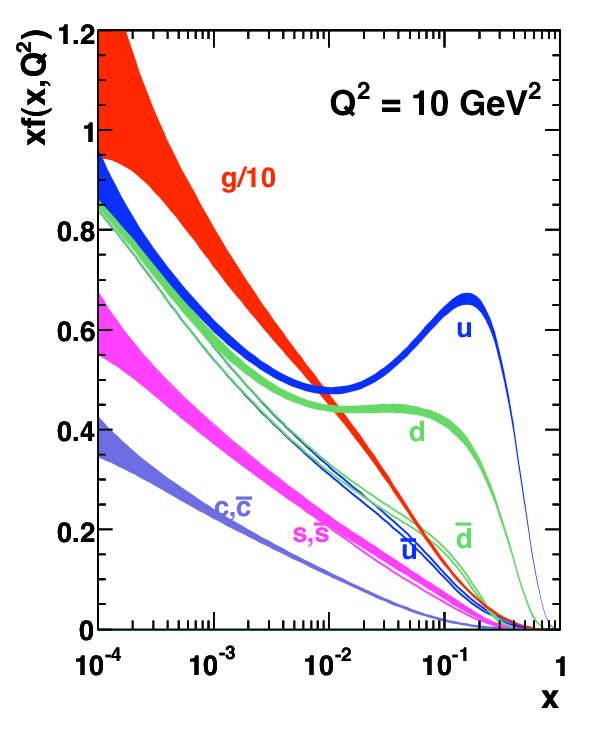
\includegraphics[width=.5\columnwidth]{Images/PDF.png}
  \center  \caption{Proton PDFs for the quark, gluon and anti-quark densities at $Q^2 = 10$GeV$^2$ as a function of the longitudinal momentum fraction x obtained by the MSTW 2008 collaboration, where the coloured bands represent the PDF uncertainty.}
    \label{PDF}
\end{figure}



\section{\label{sec3}Gluon Fusion at LO}

\begin{figure}[ht]
    \centering
    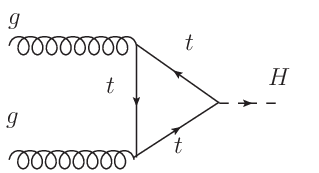
\includegraphics[width=.5\columnwidth]{Images/ggFDiagram.png}
    \caption{The first Feynman diagram for the ggF process using top quarks}
    \label{ggF diagram}
\end{figure}

Out of the 4 main Higgs production methods at the LHC, ggF has by far the highest cross section, accounting for almost $90\%$ of the total cross section. This process relies on a quark loop, as the gluons do not directly couple to the Higgs, so it's total amplitude $\mathcal{M}_{total}$  is given by
\begin{equation}
    \mathcal{M}_{total} =  \sum_{quarks} \mathcal{M}^q,
\end{equation}
as  we must sum the amplitudes for all the quarks, furthermore, each quark has two possible diagrams, $\mathcal{M}_1^q$ and $\mathcal{M}_2^q$ , one found in figure \ref{ggF diagram},  the other being the same, but swapping the gluon lines. Since gluons are bosons, the relative sign between the diagrams is positive, and the diagrams end up having the same amplitude, so

\begin{equation}
    \mathcal{M}^q = 2 \mathcal{M}^q_1.
\end{equation}
Lastly, since gluon fusion is dominated by the top quark loop, as we will soon see, we can write
\begin{equation}
    |\overline{\mathcal{M}_{total}}|^2 \simeq |\overline{\mathcal{M}^t}|^2= 4|\overline{\mathcal{M}_1^t}|^2.
\end{equation}
For now, we will compute the amplitude for a single diagram of an arbitrary quark of mass $m$, which we will call $\mathcal{M}$.


\subsection{Computing the ggF Amplitude}

The Feynman rules for this process are :

\begin{enumerate}
    \item Incoming gluons: $\varepsilon_1^{\mu}$ $\varepsilon_2^{\nu}$;
    \item Outgoing scalar: 1;
    \item Fermion loop: -1 and integrate over the loop momentum;
    \item Fermion propagators: $i\frac{(\slashed{q}+m)}{q^2-m^2}$ ,  $i\frac{(\slashed{q}+\slashed{k}_1+m)}{(q+k_1)^2-m^2}$ and $i\frac{(\slashed{q}+\slashed{k_1}+\slashed{k_2}+m)}{(q+k_1+k_2)^2-m^2}$;
    \item Quark-Gluon vertices: $\left( -ig_s\gamma_{\mu}T^a_{jk} \right)$ and  $\left( -ig_s\gamma_{\nu}T^b_{kl} \right)$;
    \item Yukawa vertex: $\left(-i\frac{g}{2}\frac{m}{m_W}\right)$;
    \item Multiply by $\delta^{jl}$ to ensure the quark and anti-quark have the same color;
    \item Finally, multiply by $i$;
\end{enumerate}
\noindent where $~q$ is the quark loop momentum, $k_1$ and $k_2$ are the incoming gluons momenta and $m$ is the quark's mass.
So now, writing the full matrix element, we get
\small
\begin{multline}
    \mathcal{M} = -i\int \frac{d^4q}{(2\pi)^4} \varepsilon_1^{\mu}\left( ig_s\gamma_{\mu}T^a_{jk} \right)i\frac{(\slashed{q}+\slashed{k}_1+m)}{(q+k_1)^2-m^2}\left( -ig_s\gamma_{\nu}T^b_{kl} \right)\varepsilon_2^{\nu}\\ i\frac{(\slashed{q}+\slashed{k_1}+\slashed{k_2}+m)}{(q+k_1+k_2)^2-m^2}\left(-i\frac{g}{2}\frac{m}{m_W}\right)i\frac{(\slashed{q}+m)}{q^2-m^2}\delta^{jl}.
\end{multline}

\normalsize
We can simplify this to

\begin{equation}
   \mathcal{M} = \frac{1}{4\pi}\left(\sqrt{2}G_F\right)^{\frac{1}{2}}m\alpha_sTr\left(T^aT^b\right)\varepsilon_1^{\mu}\varepsilon_2^{\nu}\int \frac{d^4q}{i\pi^2}\frac{T_{\mu\nu}}{D_0D_1D_2},
\end{equation}
where $\alpha_S = \frac{g_S^2}{4\pi}$,$G_F = \frac{\sqrt{2}g^2}{8m_W^2}$, $D_0  = \left(q^2-m^2\right)$, $D_1  = \left((q+k_1)^2-m^2\right)$, $D_2  = \left((q+k_1+k_2)^2-m^2\right)$. If we explicitly write the indices of the Dirac matrices, we also find that

\begin{equation} \label{DiracTrace}
    T_{\mu\nu} = \mathrm{Tr}\left[(\slashed{q}+m)\gamma_{\mu}(\slashed{q}+\slashed{k}_1+m)\gamma_{\nu}(\slashed{q}+\slashed{k_1}+\slashed{k_2}+m)\right].
\end{equation}

Since gluons are massless, they have only transverse components, therefore we can introduce the transverse projector,  $P_{T\mu\nu} = \eta_{\mu\nu} - \frac{k_{1\mu}k_{2\nu}}{k_1.k_2}$, without losing any information, so now we can write the amplitude as

\begin{equation}
    \mathcal{M} = \frac{1}{4\pi}\left(\sqrt{2}G_F\right)^{\frac{1}{2}}m\alpha_sTr\left(T^aT^b\right)\varepsilon_1^{\mu}\varepsilon_2^{\nu} F P_{T\mu\nu},
\end{equation}
where

\begin{equation}
    F = \frac{1}{4}P_T^{\mu\nu}\int \frac{d^4q}{i\pi^2}\frac{T_{\mu\nu}}{D_0D_1D_2}.
\end{equation}

The spin averaged sum for this diagram is

\begin{equation}
    |\overline{\mathcal{M}}|^2 = \frac{1}{2.2.8.8}\frac{1}{16\pi^2}\alpha_S^2\left(\sqrt{2}G_F\right)m^2\sum_{pol.}\sum_{a,b=1}^8 \left|\frac{\delta^{ab}}{2}\varepsilon_1^{\mu}\varepsilon_2^{\nu} F P_{T\mu\nu}\right|^2.
\end{equation}

%\begin{equation}
   % \sum_{pol.}\left|\varepsilon_1^{\mu}\varepsilon_2^{\nu} P_{T\mu\nu}\right|^2 = \sum_{pol.}\varepsilon_1^{\mu}\varepsilon_2^{\nu} P_{T\mu\nu}\varepsilon_1^{*\alpha}\varepsilon_2^{*\beta} P_{T\alpha\beta} = P_{T\mu\nu}P_T^{\mu\nu} = 2
%\end{equation}

The second half of the expression reduces to
\begin{equation}
    \sum_{pol.}\sum_{a,b=1}^8 \left|\frac{\delta^{ab}}{2}\varepsilon_1^{\mu}\varepsilon_2^{\nu} F P_{T\mu\nu}\right|^2=
    \sum_{a=1}^8\left(\frac{2\delta^{aa}}{4}F^2\right) = 4F^2,
\end{equation}
so now the final expression for the total amplitude squared  is given by
\begin{equation}
    |\overline{\mathcal{M}}|^2  = \frac{\sqrt{2}G_F\alpha_S^2}{32^2\pi^2}m^2F^2,
\end{equation}
now we just need to compute $F$. First we have to compute the trace in Eq.~~\ref{DiracTrace}, obtaining
\begin{multline}
    T^{\mu\nu} = 4m\left[ 4q^\mu q^\nu+2q^\mu k_1^\nu+4q^\nu k_1^\mu+2q^\nu 
    k_2^\mu \right. \\\left. +2k_1^\mu k_1^\nu+k_1^\mu k_2^\nu+k_1^\nu k_2^\mu 
    +\eta^{\mu\nu}\left(m^2-q^2-2q.k_1-k_1.k_2-k_1^2 \right)\right].
\end{multline}

The integral in (20) gives a finite result for the Higgs amplitude at LO. However, the tensor integrals present in (20) contain UV divergences in intermediate steps of the calculation that will cancel in the final result. For this reason we employ a consistent regularisation procedure called Conventional Dimensional Regularization (CDR) and perform the evaluation of the integral in $d=4-2\epsilon$ space-time dimensions to keep track of the singular terms that will cancel in the final result at which point we can take the $\epsilon \rightarrow 0$ limit.  

Contracting $T^{\mu\nu}$ with the transverse projector, keeping in mind that $k_1^2=k_2^2=0$ and $2k_1k_2 = m_H^2$, we get


\small

\begin{multline}
     P_{T\mu\nu}T^{\mu\nu} = 4m\left((d-1)m^2+\frac{(2-d)}{2}m_H^2-\frac{8}{m_H^2}k_1.q k_2.q\right. \\\left. +(6-2d)k_1.q+(5-d)q^2 \right) .
\end{multline}
   

\normalsize

To compute this integral, we need to use a technique called Passarino Veltman reduction, doing so gives us

\begin{equation}
    F=m\left(2\epsilon B_0(k_1+k_2,m)+(4m^2-m_H^2)C_0(k_1,k_2,m) \right),
\end{equation}
where $B_0$ is the UV divergent scalar two point function, 

\begin{multline}
    B_0(k_1+k_2,m) = \int \frac{d^dq}{(2\pi)^d} \frac{1}{(q^2-m^2)} \frac{1}{((q+k_1+k_2)^2-m^2)} = \\ (\frac{\mu^2}{m^2})^{\epsilon}(\frac{1}{\epsilon} + 2 - \beta \ln (\frac{1+\beta}{1-\beta})),
\end{multline}
which is multiplied by the $\epsilon$-regulator giving a finite contribution to the amplitude, and $C_0$ is the finite scalar three point function, 
\begin{equation}
    C_0(k_1,k_2,m) = \begin{cases}
            -\frac{2}{m_H^2}\arcsin^2{\left(\sqrt{\frac{1}{\rho}} \right)}  ,& \rho > 1  \\
             \frac{1}{m_H^2}\left(\log\left( \frac{1+\sqrt{1-\rho}}{1-\sqrt{1-\rho}}\right)-i\pi \right)^2,& \rho < 1,
            \end{cases}
\end{equation}
with $\rho = \frac{4m^2}{m_H^2}$. 

This gives us two different amplitude expressions, one for quarks with $\rho<1$, and one for quarks with $\rho>1$. These expressions can be simplified to be



\begin{equation}
    |\overline{\mathcal{M}}|^2 = \frac{\sqrt{2}G_F\alpha_S^2m_H^4}{64^2\pi^2}A\left(\rho\right),
    \label{FullAmpSquare}
\end{equation}
where $A\left(\rho\right)$ is given by

\begin{equation}
    A\left(\rho\right) = \begin{cases}
    
            \rho^2\left( 1+(1-\rho)\arcsin^2{\left(\sqrt{\frac{1}{\rho}} \right)}\right)^2  ,& \rho > 1  \\
            
            \rho^2\left( 1-\frac{1}{4}(1-\rho)\left| \log\left( \frac{1+\sqrt{1-\rho}}{1-\sqrt{1-\rho}}\right)-i\pi \right|^2\right)^2,& \rho  < 1 .
            \end{cases}
\end{equation}

Since the quarks in this process are all virtual, they have no effect on the phase space of the problem, so the cross sections for different quarks are directly proportional to the amplitude, which in turn is proportional to $A\left(\rho\right)$.

\begin{figure}[ht]
    \centering
    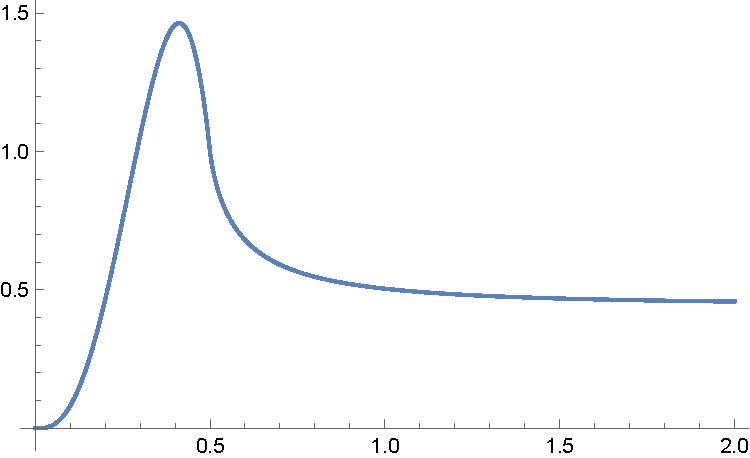
\includegraphics[width=.6\columnwidth]{Images/f(p).pdf}
    \caption{Plot of $A$ as a function of $\frac{m}{m_H}$ for quark masses from $0$ to $2m_H$ }
    \label{fp}
\end{figure}
From figure \ref{fp}, we can clearly see that light quarks contribute much less to the cross section than more massive quarks. In fact, computing the ratio between the top quark and bottom quark, we get

\begin{equation}
    \frac{|\overline{\mathcal{M}^t}|^2}{|\overline{\mathcal{M}^b}|^2} \simeq 150,
\end{equation}
while the remaining quarks contribute even less than the bottom quark. This confirms that to a first order approximation we can neglect the effects of all lighter quarks, including the top-bottom interference contribution, and therefore, the total amplitude at LO becomes 
\begin{multline}
    |\overline{\mathcal{M}_{total}}|^2 \simeq |\overline{\mathcal{M}^t}|^2= 4|\overline{\mathcal{M}_1^t}|^2 \\ = \frac{\sqrt{2}G_F\alpha_S^2m_H^4}{32^2\pi^2}\rho^2\left( 1+(1-\rho)\arcsin^2{\left(\sqrt{\frac{1}{\rho}} \right)}\right)^2 .
\end{multline}

We can also see what would happen if we added a new, fourth generation quark doublet to the Standard Model. Experiments from the LHC show that a new generation of quarks, that behave like the other SM quarks, should have a mass upwards of $1$ TeV \cite{CMS:2019eqb}. Therefore, these new quarks, $q_1 $ and $q_2$, are much heavier than the Higgs boson, and we can study what happens to the amplitude in the case that $\rho \rightarrow \infty$. Taking the limit, we get
\begin{multline}
    \lim_{\rho\rightarrow\infty} \rho\left( 1+(1-\rho)\arcsin^2{\left(\sqrt{\frac{1}{\rho}} \right)}\right) \\  =  \lim_{\rho\rightarrow\infty} \rho\left[1+(1-\rho)\left(\frac{1}{\rho}+\frac{1}{3\rho^2}\right) \right] + \mathcal{O}\left(\frac{1}{\rho}\right) = \frac{2}{3},
\end{multline}
therefore,

\begin{equation}
    \lim_{\rho\rightarrow\infty} A\left(\rho\right) = \frac{4}{9}.
\end{equation}

If we now compared the amplitude for these quarks to the top quark, we find that they are quite similar, with $|\overline{\mathcal{M}^{q_1}}|^2 = |\overline{\mathcal{M}^{q_2}}|^2  \simeq 0.94|\overline{\mathcal{M}^t}|^2$. If we make the approximation that the 4th generation quarks couple in the same way to the Higgs boson as the top quark, then the total amplitude would now become 
\begin{equation}
    \mathcal{M}'_{total} =  \sum_{quarks} \mathcal{M}^q \simeq \mathcal{M}^t+\mathcal{M}^{q_1}+\mathcal{M}^{q_2}\simeq 3\mathcal{M}^t = 3\mathcal{M}_{total},
\end{equation}

which results in an amplitude squared equal to

\begin{equation}
     |\overline{\mathcal{M}´_{total}}|^2 =  9|\overline{\mathcal{M}_{total}}|^2.
\end{equation}
Since gluon fusion currently makes up 90\% of the total Higgs production cross section, this would result in a total cross section about eight times larger than what we currently measure, seemingly ruling out the existence of these quarks. However, it is still possible to introduce fourth generation quarks while still complying with this constraint imposed by ggF.

The Yukawa coupling to up-like quarks is known to be positive \cite{Cheung_2019} , however, it is not known whether it is positive or negative for down-like quarks. If this coupling were to be negative, then we would have that $\mathcal{M}^{q_1} = -\mathcal{M}^{q_2}$, meaning that 

\begin{equation}
    \mathcal{M}'_{total} =  \sum_{quarks} \mathcal{M}^q \simeq      \mathcal{M}^t+\mathcal{M}^{q_1}+\mathcal{M}^{q_2}= \mathcal{M}^t =    \mathcal{M}_{total},
\end{equation}
and the ggF cross section would remain unchanged despite the existence of hypothetical heavy 4th generation quarks”.

\subsection{Cross Section at LO}

What we have computed so far is only for the partonic process. In reality, at the LHC, we have two protons colliding, and inside these protons is where we find the gluons. These gluons can carry varying portions of the total proton momentum. The total hadronic cross section is given by

\begin{equation}
    \sigma_{total} = \int\int dx_1dx_2 f\left(x_1\right)f\left(x_2\right)\sigma_{part},
\end{equation}
where $x_1$, $x_2$ are momentum fractions carried by each gluon, and $f\left(x\right)$ is the gluon parton distribution function.  If we write each gluons' momentum as $k = xP$, $P$  being the protons momentum, we find that

\begin{equation}
    s = (k_1+k_2)^2 =(x_1P_1+x_2P_2)^2  = 4x_1x_2E^2 = x_1x_2S,
\end{equation}
$S$ being the center of mass energy of the proton collision. Here we have ignored the proton's mass, as its energy in colliders  is always much larger than its mass.

The parton cross section is 
\begin{equation}
    \sigma_{part} =\frac{1}{2s} \int \frac{d^3p}{(2\pi)^32p_0}(2\pi)^4 |\overline{\mathcal{M}_{total}}|^2 = \frac{\pi}{m_H^2}\delta\left(s-m_H^2\right)|\overline{\mathcal{M}_{total}}|^2.
\end{equation}

From now, it will be useful to do a variable change from $x_1$ and $x_2$, to $x = x_1x_2$ and $y = \frac{1}{2}\log(\frac{x_1}{x_2})$. Now, $x_1 = \sqrt{x}\exp(y)$, $x_2 = \sqrt{x}\exp(-y)$, $dx_1dx_2 = dxdy$, and $s = xS$. The total hadronic cross section now becomes
\begin{multline}  
    \sigma_{total} = \frac{\pi}{m_H^2}|\overline{\mathcal{M}_{total}}|^2  \int\int dx~dy~ f\left(\sqrt{x}\exp(y)\right) \\ \times f\left(\sqrt{x}\exp(-y)\right)\delta\left(xS-m_H^2\right).
\end{multline}

Using the identity $\delta(\alpha x) = \frac{1}{|\alpha|}\delta(x)$ and simplifying, we arrive at

\begin{equation}
     \sigma_{total} = \frac{\sqrt{2}G_F\alpha_S^2m_H^2}{32^2\pi S}A\left(\rho\right) \int dy~ f\left(\sqrt{x_0}\exp(y)\right)f\left(\sqrt{x_0}\exp(-y)\right),
\end{equation}
with $x_0 = \frac{m_H^2}{S}$.

In order to obtain a numerical value for the cross section, we now have to integrate over the PDFs. This, however, cannot be done by hand, and we must use a program to do this calculation for us, for this project, we chose to use Ihixs2 \cite{Dulat_2018}. This program computes the LO cross section with the full top quark mass dependence in the loop and makes use of an effective field theory in order to simplify the calculation of higher order QCD corrections to the Higgs cross section.


\subsection{Effective Field Theory}
    
    In order to build the effective field theory, we can take the limit as the quark mass approaches infinity, where the ggF interaction would behave as a point-like interaction. We can write the point interaction amplitude like this

    \begin{equation}
    \mathcal{M} = \mathcal{K}\,Tr\left(T^aT^b\right)\varepsilon_1^{\mu}\varepsilon_2^{\nu} P_{T\mu\nu},
    \label{EFF amp}
\end{equation}
where we need to find what $\mathcal{K}$ is. Squaring and summing this amplitude we get

\begin{equation}
    |\overline{\mathcal{M}}|^2 = \frac{1}{2.2.8.8}\mathcal{K}^2\sum_{pol.}\sum_{a,b=1}^8 \left|\frac{\delta^{ab}}{2}\varepsilon_1^{\mu}\varepsilon_2^{\nu} P_{T\mu\nu}\right|^2=\frac{1}{64}\mathcal{K}^2,
\end{equation}

now we just need to make sure it is equal to equation \ref{FullAmpSquare} in the large mass limit, with $A\left(\rho\right) = \frac{4}{9}$, so
\begin{equation}
    \frac{1}{64}\mathcal{K}^2 = \frac{\sqrt{2}G_F\alpha_S^2m_H^4}{64^2\pi^2}\frac{4}{9} \implies \mathcal{K}=\frac{ (\sqrt{2}G_F) ^{\frac{1}{2}} }{12\pi}m_H^2\alpha_S.
\end{equation}

And the vertex for the effective field theory can be written by removing the incoming gluons from equation \ref{EFF amp}, obtaining
\begin{equation}
    \sim \frac{ (\sqrt{2}G_F) ^{\frac{1}{2}} }{12\pi}m_H^2\alpha_S Tr\left(T^aT^b\right)P_{T\mu\nu}.
\end{equation}

Using this vertex, we can compute the ggF amplitude in the large mass limit, simplifying higher order calculations. But as we have seen before, the amplitude for the top quark diagrams is slightly higher than the large mass limit, with $|\overline{\mathcal{M}^{q}}|^2  \simeq 0.94|\overline{\mathcal{M}^t}|^2$, meaning that, after performing the calculation using the effective field theory, we will rescale all higher order effective theory cross sections by the ratio $R_{LO} = \sigma_{LO}^t /\sigma_{LO}^{EFT}$, the ratio between the exact LO result with top quark mass dependence over the LO result in the infinite top-mass limit, which multiplies our result by ≈ 1.06 and accounts for the finite top quark mass effects in the cross section. This recalling factor is also already implemented into the ihixs2 code. 

\section{\label{sec4}Numerical Results}

Before computing the numerical results,  we must define some constants when running the program. The mass of the Higgs boson we simply set to $125$GeV, but we must also set the renormalization $\mu_R$ and factorization $\mu_F$ scales, as these represent the energy scales at which we will evaluate the strong coupling constant $\alpha_S$ , and the PDFs, respectively. Each of these quantities will vary depending on the energy level at which they are probed, for this project, we chose to set both of them to $62.5$GeV, half of the mass of the Higgs boson, as a good middle ground for the energy level of the process involved in ggF.  To estimate the theory uncertainty from this assignment will consider variations of $\mu_R$ and $\mu_F$ up and down this central value by a factor of 2 and consider the envelope of all Higgs cross section values inside this variation as an uncertainty band.

There are many PDF sets, all developed by different teams around the world. Ihixs2 lets us to choose the PDF we want, allowing us to compare results with different PDFs.

The first set of results uses the same PDF, NNPDF40, to compute the Higgs cross section at increasing center of mass energy values, from $7$TeV to $100$TeV. 

\begin{figure}[ht]
    \centering
    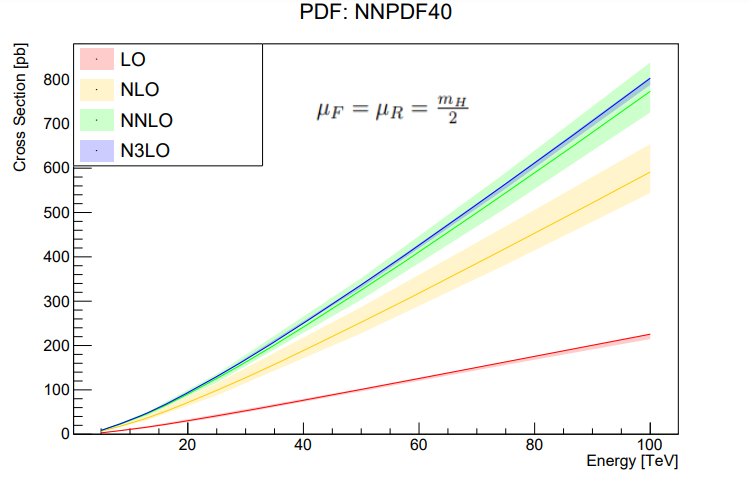
\includegraphics[width=.8\columnwidth]{Images/NNPDFXS.png}
    \caption{ Plot of the Higgs cross section in picobarns [pb] as a function of the center of mass collision energy [TeV]. The shaded bands at each order show the perturbative $\mu_R$ and $\mu_F$ scale uncertainty. }
    \label{results1}
\end{figure}
From figure \ref{results1}, two things stand out. Firstly, the cross section increases more than linearly with the collider energy, being around twenty times larger at $100$TeV than it is at the current $13$TeV in the LHC.

Secondly, the LO approximation is very inaccurate, as it seems to only account for about one quarter of the total cross section. This is the result of two facts. The first being that for higher order processes in QCD beyond LO new channels open up, for example the quark-gluon channel that appears for the first time at NLO with additional diagrams to take into account. Second, the strong coupling constant $\alpha_S$ is relatively large compared to the other interactions, being about $\sim0.1$ at these energy scales, making it so that the perturbative expansion for Higgs production has a slow convergence. This results in a large increase in the value of the Higgs cross section when going from LO to NLO and to NNLO, where in particular we can see in the Figure that the uncertainty bands of each perturbative prediction do not overlap. The exception to this observation is the N3LO Higgs cross section prediction that for the first time exhibits a perturbative scale uncertainty band that is within the NNLO band.

We can do a second plot which shows this more clearly.

\begin{figure}[ht]
    \centering
    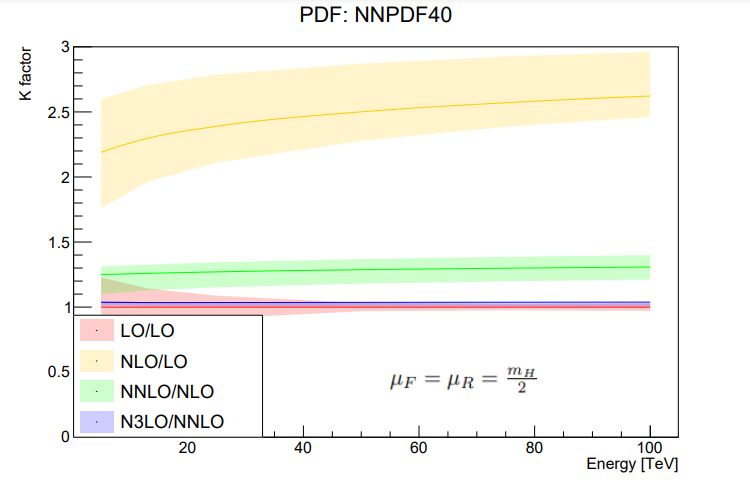
\includegraphics[width=.8\columnwidth]{Images/NNPDF40K.png}
    \caption{Perturbative QCD corrections at NLO (yellow), NNLO (green) and N3LO (blue) to the Higgs ggF cross section as a function of the center of mass collision energy [TeV]. }
    \label{results2}
\end{figure}


In figure \ref{results2} we plot the ratio of the Higgs cross sections from a higher order in QCD to a lower one as a function of $\sqrt{S}$. Here we can see clearly that with respect to the LO result, the NLO result (in yellow) is larger by a factor of $2.2\sim2.5$ and the NNLO corrections (in green) increase it further by approximately 30\%. Finally we also see that the N3LO correction changes the cross section by about 2\%, meaning that higher order terms in the perturbative expansion are probably negligible. From the same Figure we can observe a dramatic reduction in the theory uncertainty of the Higgs cross section as determined by the width of bands in the plot. At NNLO the theoretical scale uncertainty is approximately 15\% (a factor of 2 smaller than the NLO scale dependence), while at N3LO this theoretical uncertainty is at the 3\% level.  At this level of accuracy it becomes non-negligible the inclusion of Electroweak corrections and quark mass effects to the inclusive Higgs production cross section.


After the phenomenological study of the ggF Higgs cross section we can now show the comparison between the theory predictions that were obtained and the measurements performed at the LHC by the ATLAS\cite{ATLAS:2019nkf} and CMS\cite{CMS:2021ugl} experiments.

\begin{figure}[ht]
    \centering
    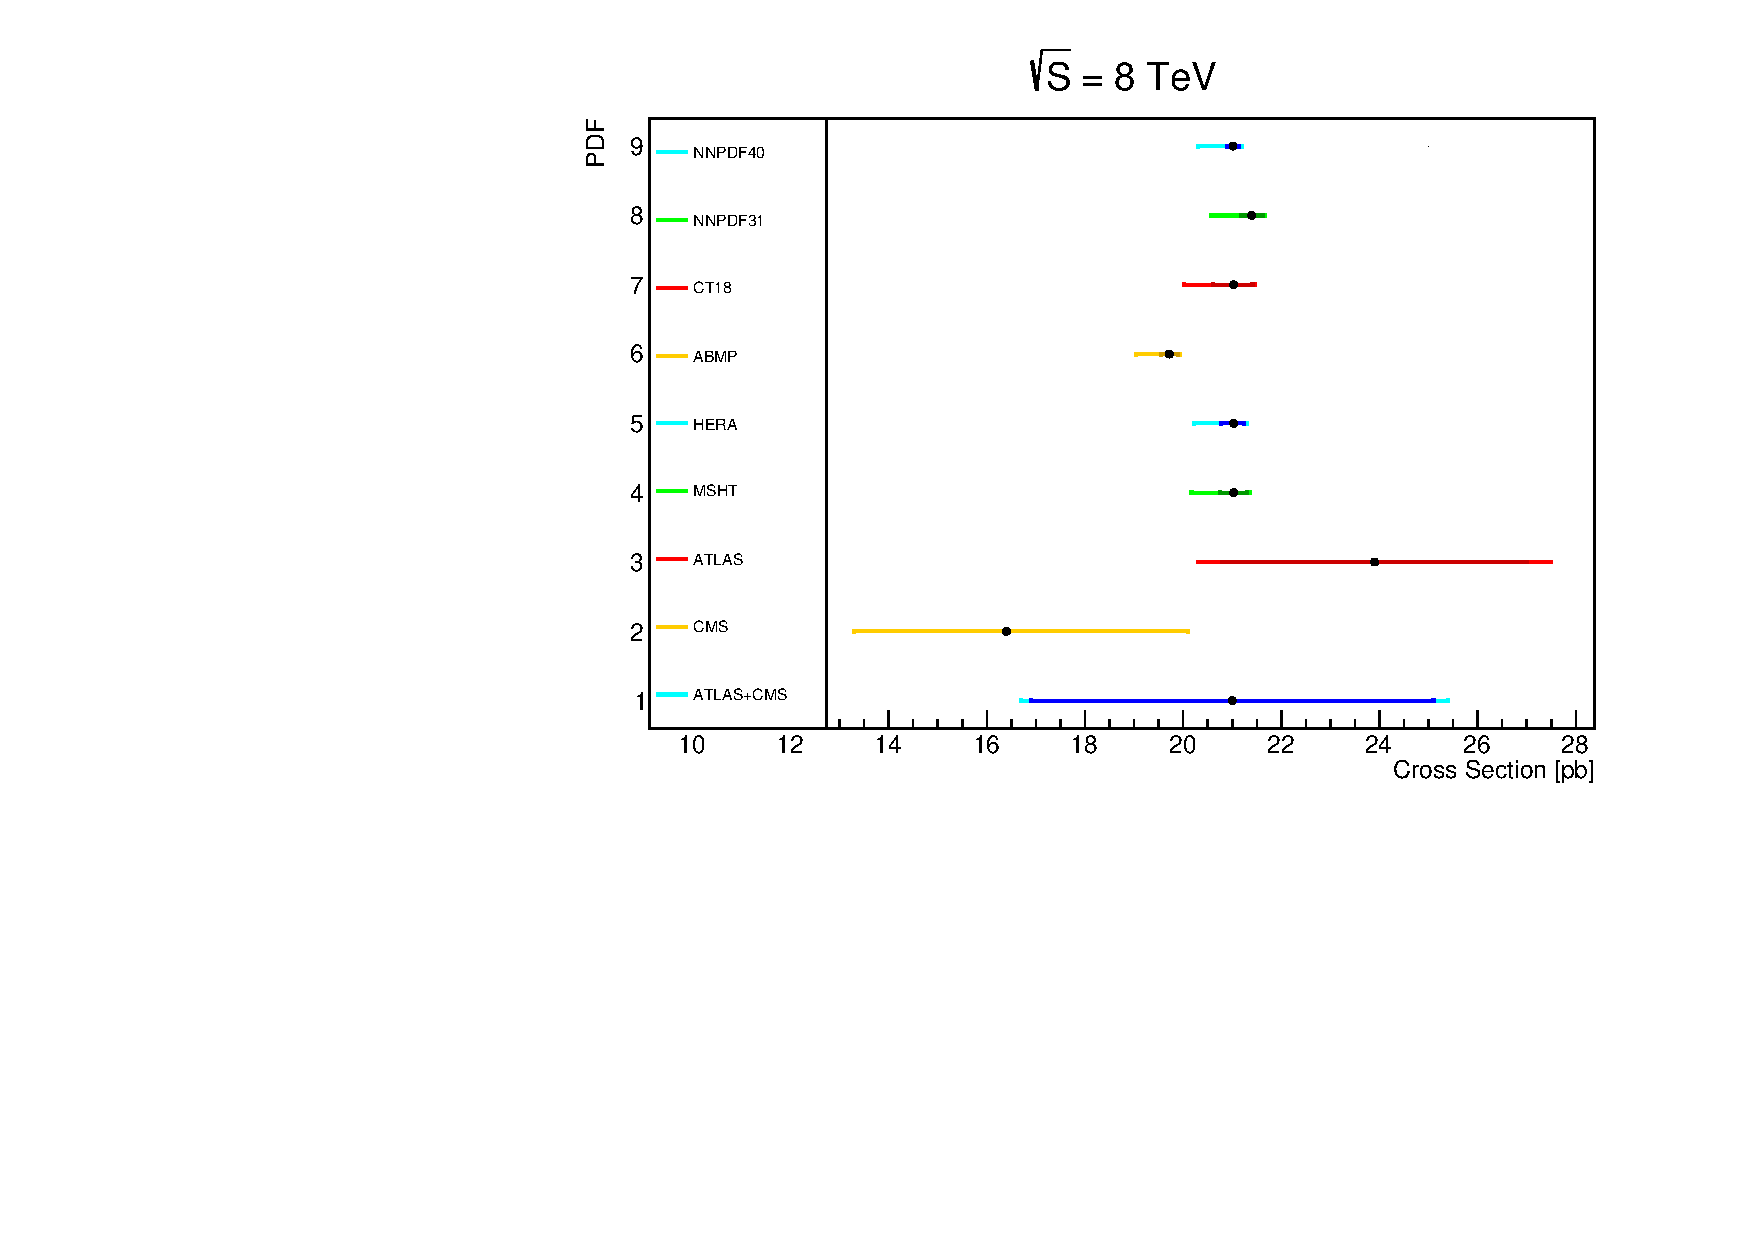
\includegraphics[width=.8\columnwidth]{Images/Graph2.pdf}
    \caption{Plot of the N3LO ggF Higgs cross section in picobarn [pb] for various PDFs for proton-proton collisions at a center of mass energy $\sqrt{s}= 8$TeV and experimental results from ATLAS\cite{ATLAS:2015egz}  and CMS\cite{CMS:2014fzn}  and their combination\cite{ATLAS:2016neq} . }
    \label{results3}
\end{figure}

\begin{figure}[H]
    \centering
    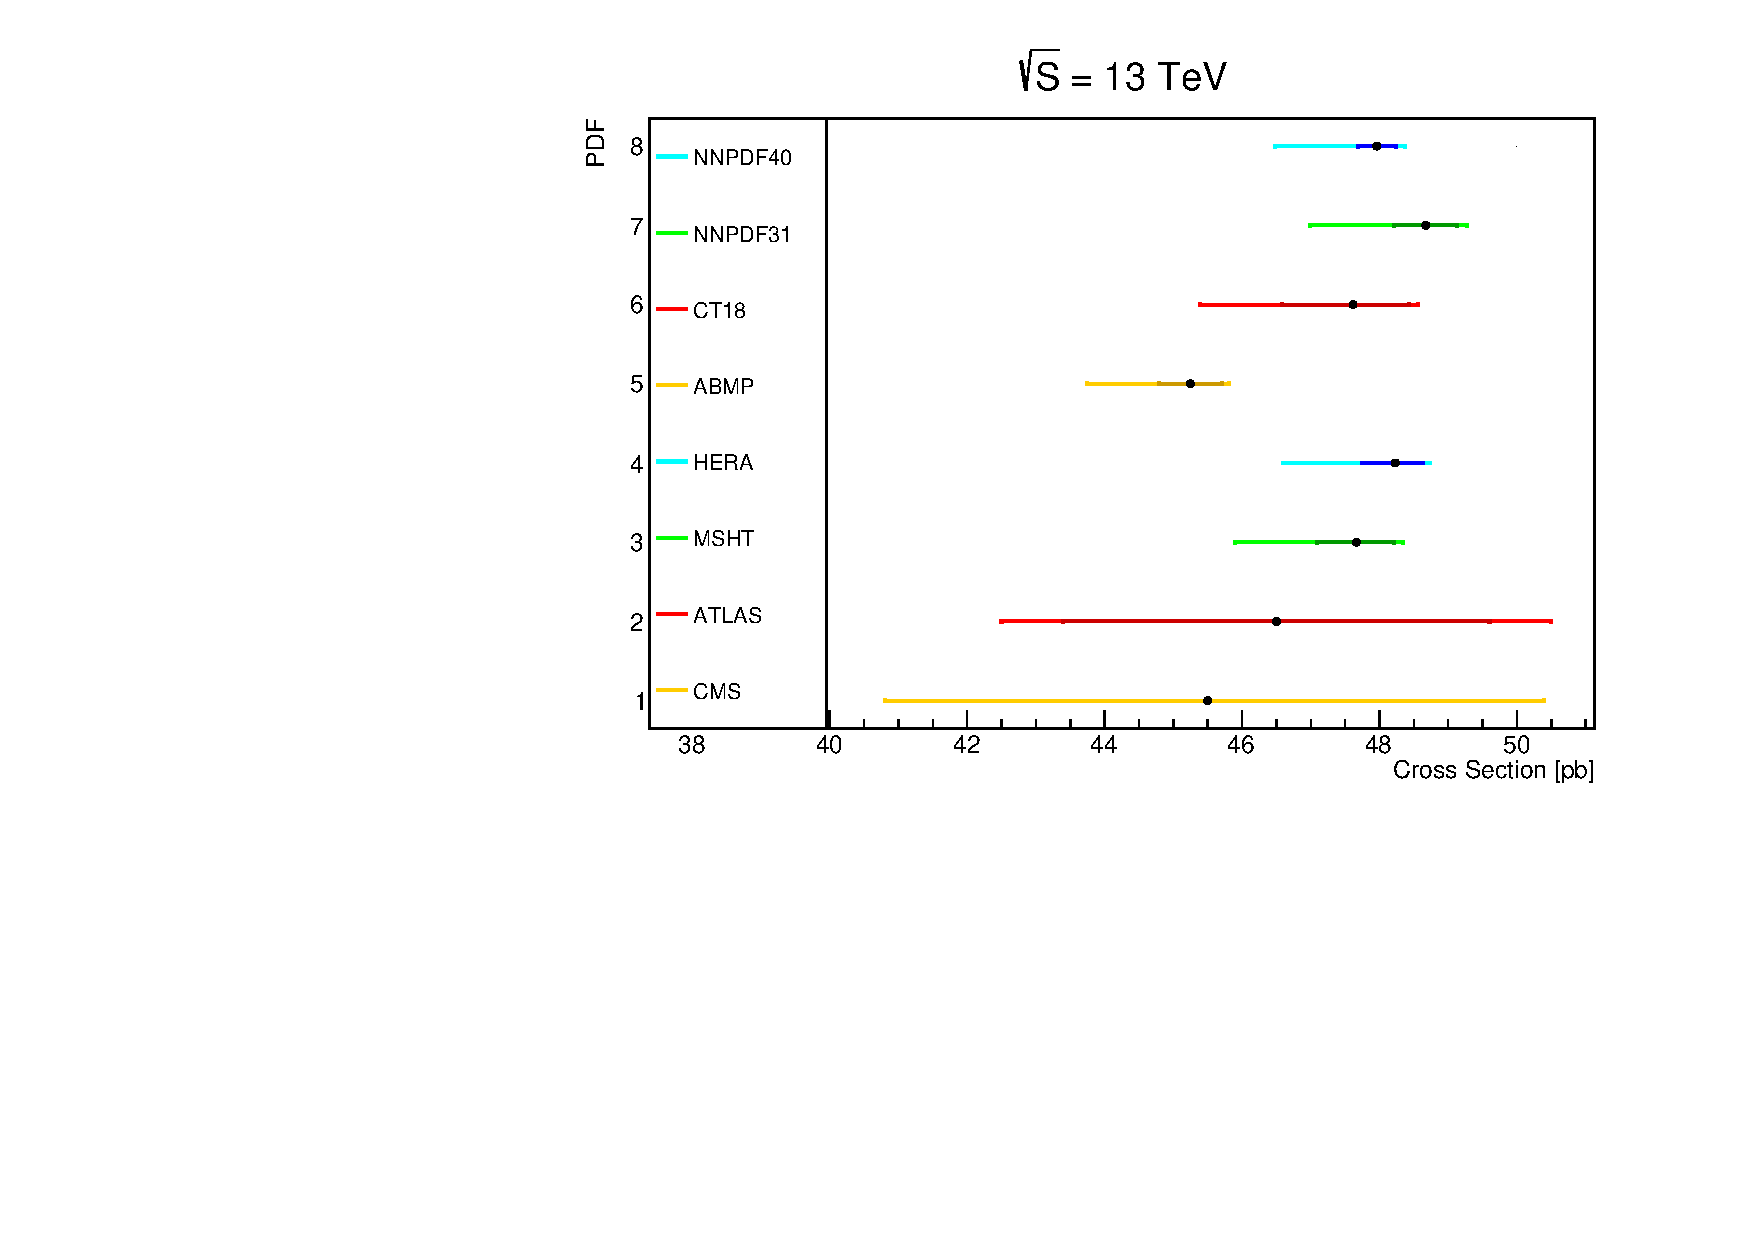
\includegraphics[width=.8\columnwidth]{Images/Graph3.pdf}
    \caption{Plot of the N3LO ggF Higgs cross section in picobarn [pb] for various PDFs for proton-proton collisions at a center of mass energy $\sqrt{s}= 13$TeV and experimental results from ATLAS\cite{ATLAS:2019nkf}  and CMS\cite{CMS:2021ugl} .}
    \label{results4}
\end{figure}

To do this we plot in figures \ref{results3} and \ref{results4}, the ggF Higgs cross section computed at N3LO in proton-proton collisions at $\sqrt{S}=8$ TeV and $\sqrt{S}=13$ TeV using different NNLO PDF sets as well as the ATLAS and CMS experimental results from the LHC. Here, in the case of the numerical results, the darker error bars represent the uncertainty due to the PDFs and the lighter error bars represent the total uncertainty, as for the experimental results, the error bars represent the statistical and the total uncertainty, respectively.

We find that the predictions using different PDF sets mostly agree with each other, the only outlier being ABMP which has a softer gluon distribution and predicts a lower Higgs cross section. In conclusion we can see that the prediction of the Standard Model for the ggF Higgs cross section at N3LO agrees well with the experimental results, mostly due to the fact that the error bars on the experimental results are still quite large $\mathcal{O}(12\%)$.

Finally, we can also compare how the Future Circular Collider (FCC) compares to the LHC in terms of producing Higgs bosons. During the first run of the LHC, it ran at an energy of $7$TeV with an integrated luminosity of $4.8$ fb$^{-1}$, and and an energy of $8$TeV, with a luminosity of $20.7$ fb$^{-1}$. An experimentally clean way of detecting Higgs bosons is through the $H\rightarrow\gamma\gamma$ decay channel, with a branching ratio of $0.2\%$, this mean we can calculate the number of expected events during the first run
\small
\begin{equation*}
         N_{H\rightarrow\gamma\gamma} = BR_{H\rightarrow\gamma\gamma} \times\left[\sigma_{7TeV} \times 4.8fb^{-1} + \sigma_{8TeV} \times 20.7fb^-1\right] \approx 1000.   
\end{equation*}

There is also the LHC high luminosity run (HL-LHC)\cite{Styles:2015svq}, which will be running from 2029 to 2040, with a total integrated luminosity of $\approx 3000$fb$^{-1}$ at a center of mass energy of $\sqrt{S} = 14$TeV. So, in one year, we should expect a number of events equal to

\small
\begin{equation*}
         N_{H\rightarrow\gamma\gamma} = BR_{H\rightarrow\gamma\gamma} \times\left[\sigma_{14TeV} \times \frac{3000}{11}fb^{-1}\right] \approx 2.5\times 10^4.
\end{equation*}

\normalsize
As for the FCC, the estimated annual integrated luminosity  is of $0.2-2$ ab$^{-1}$ \cite{Zimmermann:IPAC2016-TUPMW037}, doing the same calculation as before, we get
\small
\begin{equation*}
         N_{H\rightarrow\gamma\gamma} = BR_{H\rightarrow\gamma\gamma} \times\left[\sigma_{100TeV} \times (0.2-2)ab^{-1}\right] \approx (0.3-3.2) \times 10^6.
\end{equation*}
     
\normalsize
That is potentially one hundred times more $H\rightarrow\gamma\gamma$ events per year than the LHC! 

This large increase in the number of events should reduce the statistical error by a factor of 10, allowing for more precise measurements,  give us better statistics on the kinematics of the Higgs' final state, and allow us to see rarer decay channels which cannot be found in the LHC. Such a collider would definitely reveal many more insights into the behaviour of the Higgs boson.~


\section{\label{sec5}Conclusions}
We have studied the production process of the Higgs boson, being able to obtain an expression for the gluon fusion cross section, as well as obtain numerical results using Ihixs2.

Starting from the ggF LO diagram, we were able to solve the three point integral for the quark loop, and obtain an analytical expression for the squared amplitude of the ggF process, obtaining a general function capable of computing the amplitude for a general quark with any given mass. From this, we were able to prove that the top quark is the single most important contributor, allowing us to reach a simple expression for the total amplitude.

Using the expression for the amplitude, we were able to obtain the partonic cross section and, from this, and expression the total cross section for the ggF process.

We were able to formulate an effective field theory, which simplifies the computation of higher-order QCD corrections to the cross section, which were then calculated using the program Ihixs2\cite{Dulat_2018}.
The numerical results obtained allowed us to see how the cross section evolves with the collision energy, while also agreeing with the currently available experimental data.

Finally, a simple calculation was made, showing how the proposed FCC should be able to produce around 100 times more Higgs bosons per year than the LHC, which should improve our statistical accuracy, as well as allow us to observe new, previously unseen decay channels, which would surely boost the research efforts into this very important piece of the standard model.

Although the gluon fusion is the most important contribution to the Higgs cross section, in the future, a more detailed study should also focus on the other production processes, as they still account for around $10\%$ of the total cross section. Additionally, the bottom quark’s squared amplitude term is negligible, being about 150 times smaller than the top quark’s, but the interference term between the top quark’s and bottom quark’s amplitude should also be numerically studied in perturbative QCD, since its effects could also be significant to reach the level of theory precision of a few percent. 

\section*{Acknowledgements}
I would like to thank João Pires, the supervisor of this project, for his assistance during this internship, as well as LIP for this opportunity. This project allowed me to put into practice what I have learned for the past few years, as well as learn much more particle physics, which I would not have learned in any course I have available.


\appendix 




\bibliography{BibTexFile}

\end{document}



